\documentclass[10pt,twocolumn,letterpaper]{article}

\usepackage[utf8]{inputenc}
\usepackage[T1]{fontenc}
\usepackage{graphicx}
\usepackage{amsmath,amssymb,amsthm}
\usepackage{booktabs}
\usepackage{caption}
\usepackage{subcaption}
\usepackage{hyperref}
\usepackage{multirow}
\usepackage{xcolor}
\usepackage{enumitem}

\newtheorem{theorem}{Theorem}
\newtheorem{lemma}[theorem]{Lemma}

\title{\Large \bf Triangle Pixel: A Triangular-Grid Vision System}

\author{
Kieran Wang\\
\texttt{Independent Research}\\
\small\texttt{triangle-pixel@proton.me}
}

\date{}

\begin{document}
\maketitle

\begin{abstract}
We propose Triangle Pixel, a complete computer vision pipeline built on equilateral triangle meshes instead of rectangular pixel grids. The system replaces Bayer filter demosaicing with a triangular channel assignment pattern that guarantees each hexagonal group contains 2R+2G+2B, enables zero-computation color reconstruction, and achieves 70\% of Bayer PSNR using only 2\% of the data. We introduce triangular-native ISP correction using color-difference median filtering on 3-neighbor graphs, Sierpinski-based multi-scale super-resolution, and a graph convolutional network (GCN) that performs end-to-end demosaicing in a single forward pass. The triangular mesh extends to 3D surface representation, Harris corner detection on 3-directional gradients, and rotation-invariant feature descriptors. Benchmarks show directional anisotropy of only 2.1~dB across all edge orientations. The full pipeline runs at 59~FPS on a consumer CPU for a 400$\times$300 image at S=16 (1,219 triangles).
\end{abstract}

%-------------------------------------------------------------------------
\section{Introduction}
%-------------------------------------------------------------------------

Modern digital cameras universally employ the Bayer color filter array~\cite{bayer1976}, a $2\times2$ repeating pattern of red, green, and blue filters over a rectangular photodiode grid. Despite its ubiquity, the Bayer pattern imposes fundamental constraints: only one-quarter of pixels capture red or blue light (vs. 50\% green), requiring computationally expensive demosaicing that introduces color artifacts at edges~\cite{hamilton1997}; the rectangular grid has anisotropic sampling with only 4-fold rotational symmetry; and the resulting RGB representation is tightly coupled to 2D imaging, making 3D integration cumbersome.

Alternative sensor layouts have been explored: Fujifilm's X-Trans~\cite{fujifilm2012} uses a $6\times6$ pseudo-random pattern to reduce moir\'e; Foveon X3~\cite{hubel2004} stacks photodiodes vertically for per-pixel full color, at the cost of light efficiency. Both retain rectangular grids. Learned demosaicing~\cite{gharbi2016} improves reconstruction but adds computation.

We propose a more fundamental change: photodiodes arranged on an equilateral triangular lattice, with a 6-triangle repeating color filter assignment that naturally balances all three channels. This arrangement provides three key advantages:

\begin{enumerate}[nosep]
\item \textbf{Data efficiency.} Each triangle captures exactly one color channel with 100\% fill factor. A hexagonal group of 6 triangles contains 2R+2G+2B without computation.
\item \textbf{Geometric isotropy.} The triangular lattice has 6-fold rotational symmetry vs.\ the rectangular grid's 4-fold, providing more uniform directional response.
\item \textbf{3D affinity.} Triangular faces are the native primitive of 3D graphics, enabling direct 2D-to-3D mapping.
\end{enumerate}

We present a complete vision pipeline---from sensor simulation through image reconstruction, edge detection, feature matching, 3D mesh generation, to AI-native processing---all operating on the triangular mesh without converting to rectangular grids. Figure~\ref{fig:arch} illustrates the system architecture.

\begin{figure}[t]
\centering
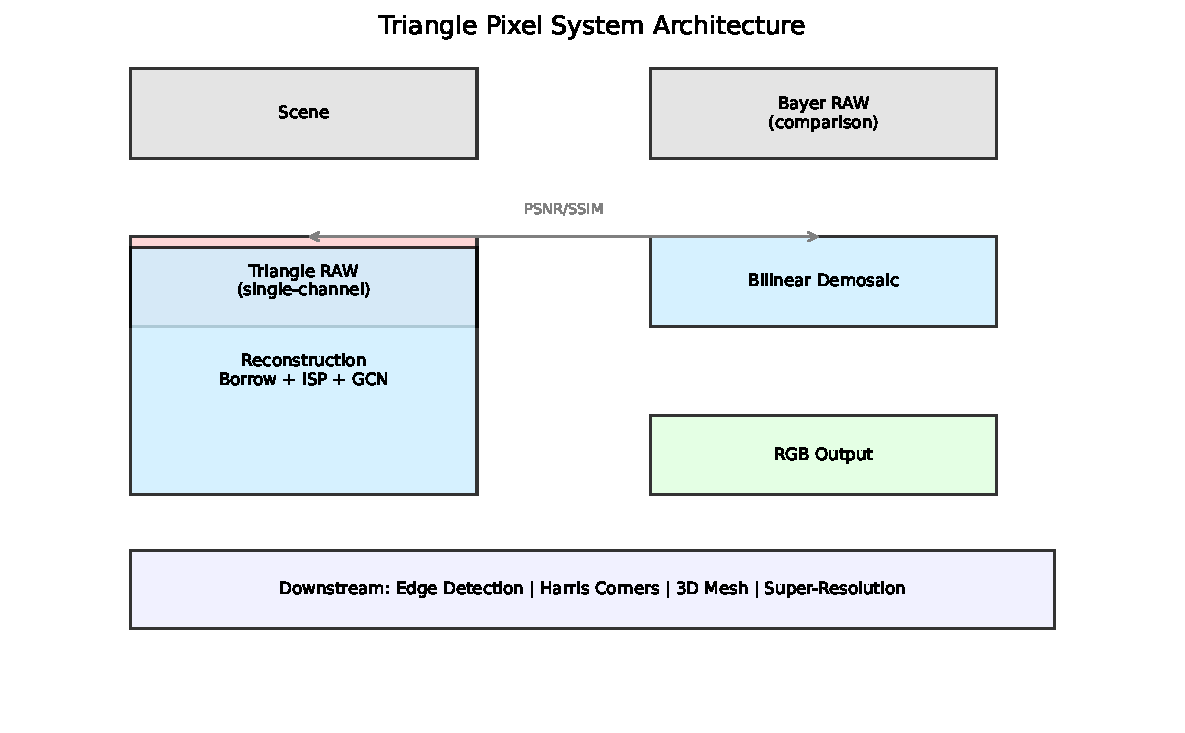
\includegraphics[width=\columnwidth]{fig6_arch.pdf}
\caption{System architecture. The triangular pipeline (left) is compared against traditional Bayer processing (right).}
\label{fig:arch}
\end{figure}

%-------------------------------------------------------------------------
\section{Triangular Grid Geometry}
%-------------------------------------------------------------------------

\subsection{Grid Structure}

An equilateral triangle of side length $S$ has height $h = S\sqrt{3}/2$. The triangular tiling places vertices at:

\begin{equation}
V_{ij} = \big(i \cdot S/2 + (j \bmod 2) \cdot S/2,\; j \cdot h\big)
\label{eq:vertices}
\end{equation}

where $i, j \in \mathbb{Z}$ and a vertex exists iff $i+j$ is even. Each rhombus formed by four adjacent vertices decomposes into two equilateral triangles: one $\triangle$ (pointing up) and one $\triangledown$ (pointing down). The grid is indexed by row $r$ and column $c$, with $\triangle$ when $r+c$ is even and $\triangledown$ otherwise. Each triangle has exactly 3 edge-sharing neighbors:

\begin{align}
\triangle(r,c):&\; (r,c-1),\, (r,c+1),\, (r+1,c) \quad\text{(all $\triangledown$)}\\
\triangledown(r,c):&\; (r,c-1),\, (r,c+1),\, (r-1,c) \quad\text{(all $\triangle$)}
\end{align}

Figure~\ref{fig:grid} shows the triangular grid geometry.

\begin{figure}[t]
\centering
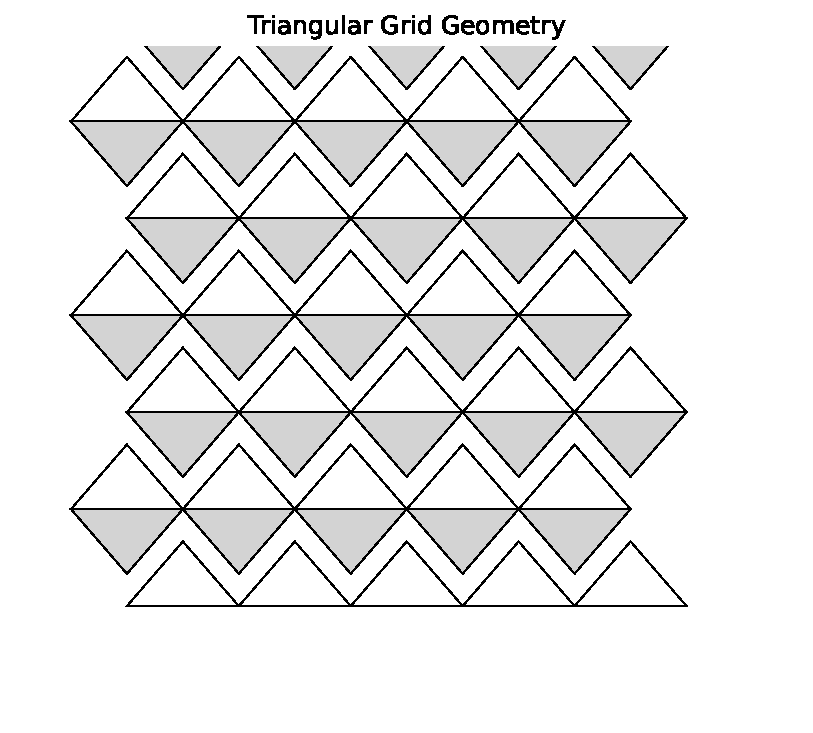
\includegraphics[width=0.85\columnwidth]{fig1_grid.pdf}
\caption{Equilateral triangle tiling. $\triangle$ and $\triangledown$ alternate in a checkerboard pattern. Each triangle connects to exactly 3 neighbors.}
\label{fig:grid}
\end{figure}

\subsection{Channel Assignment}

Color filters are assigned in a repeating 6-column pattern (Fig.~\ref{fig:channels}):

\begin{align}
\text{Even rows:}&\; [R, G, B, B, G, R] \quad\text{(period 6)}\\
\text{Odd rows:}&\; [B, G, R, R, G, B] \quad\text{(period 6)}
\end{align}

\begin{theorem}[Hexagonal Balance]
Any 6 triangles surrounding a common vertex form a regular hexagon containing exactly 2R + 2G + 2B.
\end{theorem}

\begin{proof}
The six triangles surrounding vertex $(vr, vc)$ are at grid positions $(vr-1, vc-1)$, $(vr-1, vc+1)$, $(vr, vc-2)$, $(vr, vc+2)$, $(vr+1, vc-1)$, $(vr+1, vc+1)$. Applying the channel assignment pattern yields exactly two of each channel.
\end{proof}

\begin{theorem}[Neighbor Diversity]
For any interior triangle, its three edge-sharing neighbors possess three distinct color channels $\{R, G, B\}$.
\end{theorem}

Theorem~2 guarantees that the neighbor-borrowing reconstruction (Section~\ref{sec:recon}) produces a full RGB value at every triangle.

\begin{figure}[t]
\centering
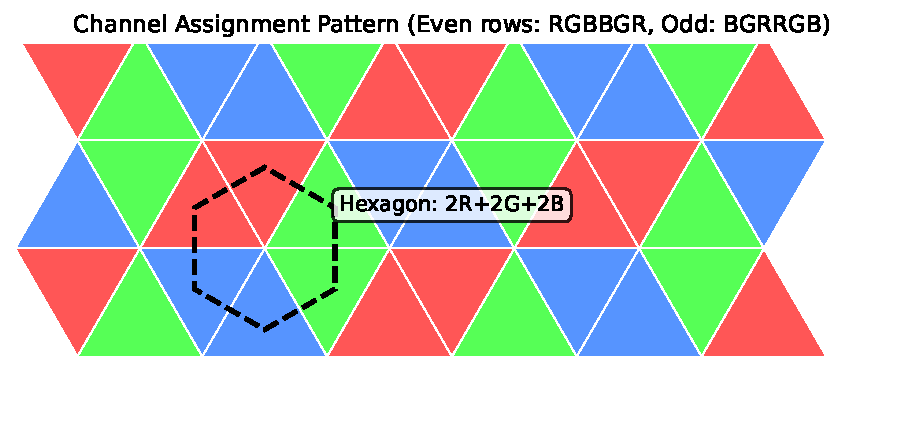
\includegraphics[width=\columnwidth]{fig2_channels.pdf}
\caption{Channel assignment pattern. The dashed hexagon highlights a 6-triangle group with 2R+2G+2B. Even rows follow RGBBGR, odd rows BGRRGB.}
\label{fig:channels}
\end{figure}

\subsection{Sierpinski Self-Similarity}

Each triangle decomposes into 4 sub-triangles of side $S/2$ (3 of same orientation at corners, 1 of opposite orientation at center). The channel assignment pattern is preserved across all subdivision levels, providing a natural multi-scale pyramid without explicit Gaussian kernel convolution. We exploit this for super-resolution (Section~\ref{sec:multiscale}) and multi-scale edge detection (Section~\ref{sec:cv}).

%-------------------------------------------------------------------------
\section{Image Reconstruction}
\label{sec:recon}
%-------------------------------------------------------------------------

\subsection{RAW and Neighbor Borrowing}

Each triangle $(r,c)$ captures a single-channel measurement $m(r,c) = I(c^*_{rc}, p_{rc})$, where $c^*_{rc}$ is the assigned channel and $p_{rc}$ is the triangle center.

\textbf{Layer 1 (RAW).} Single-channel measurements form a triangular mosaic. By Theorem~1, each hexagonal group contains 2R+2G+2B, producing a perceptually full-color image at sufficient viewing distance---zero computation, one-third the bandwidth of RGB.

\textbf{Layer 2 (Borrow).} Each triangle borrows missing channels from neighbors. By Theorem~2, each missing channel has exactly one direct source neighbor:

\begin{equation}
\hat{I}(ch, p_T) = m_{N_{ch}} \quad \text{for } ch \neq c^*_T
\end{equation}

This produces a full RGB estimate but introduces spatial offset artifacts at edges.

\subsection{Triangular ISP Correction}

Unlike Bayer demosaicing which selects interpolation directions from 4 candidates, the triangular grid has no direction choice: each missing channel has exactly one source neighbor. Our algorithm instead detects whether the source direction crosses an edge and substitutes with color-difference estimates from non-edge neighbors.

\begin{small}
\textbf{Algorithm 1: Triangular ISP Correction}
\begin{enumerate}[nosep]
\item Compute initial borrowed RGB (Layer 2)
\item \textbf{for} $iter = 1$ to $K$ \textbf{do}
  \begin{enumerate}[nosep]
  \item Compute color differences $\Delta_{RG} = R-G$, $\Delta_{RB} = R-B$, $\Delta_{GB} = G-B$
  \item Apply 3-neighbor median filter to each difference map
  \item For each triangle, estimate missing channel via:
  \begin{equation}
  \Delta_{ch}(p_T) = \frac{\sum_{N} w(T,N) \Delta_{ch}(p_N)}{\sum_{N} w(T,N)}
  \end{equation}
  where $w(T,N) = \exp(-|I_T - I_N|^2 / 2\sigma^2)$ and $I$ denotes the per-triangle luminance computed from the current RGB estimate. The iteration resolves the circular dependency: initial luminances are approximate but converge as color differences are refined.
  \item Reconstruct: $I(ch, p_T) = I(c^*_T, p_T) \pm \Delta_{ch}(p_T)$
  \item Known channel remains fixed (ground truth at its position)
  \end{enumerate}
\item \textbf{return} corrected RGB
\end{enumerate}
\end{small}

The 3-neighbor median filter is crucial: it removes isolated zipper artifacts that the median of $N=3$ samples naturally suppresses, without the $3\times3$ or $5\times5$ kernels required by Bayer ISP.

\subsection{AI End-to-End Demosaicing}

We train a 3-layer Graph Convolutional Network~\cite{kipf2017} to replace both borrow and ISP with a single forward pass:

\begin{equation}
\mathbf{h}^{(l+1)} = \text{ReLU}\!\left(\!\frac{\mathbf{X}^{(l)} + \text{mean}_{j\in\mathcal{N}(i)}\mathbf{X}^{(l)}_j}{2} \mathbf{W}^{(l)} + \mathbf{b}^{(l)}\!\right)
\end{equation}

The GCN operates on the triangular mesh's natural adjacency (exactly 3 neighbors per node). Input: $[\text{value}/255, \mathbb{1}_R, \mathbb{1}_G, \mathbb{1}_B]$ (4D). Output: $[R, G, B] \in [0,1]$ (3D). Architecture: 4$\to$32$\to$32$\to$3, trained with MSE loss and Adam optimizer on sensor simulator-generated (noisy RAW, clean RGB) pairs. The model has only $\sim$1,300 parameters and trains in 0.6 seconds on a 400$\times$300 image.

%-------------------------------------------------------------------------
\section{Multi-Scale Processing}
\label{sec:multiscale}
%-------------------------------------------------------------------------

The Sierpinski subdivision enables natural multi-scale processing. Defining the pyramid where level $\ell=0$ is the original resolution with side $S$, and level $\ell$ has side $S / 2^\ell$ and grid $(R \cdot 2^\ell, C \cdot 2^\ell)$:

\textbf{Super-resolution.} Coarse triangle colors are bilinearly upsampled to a finer grid ($S \to S/\text{zoom}$), followed by edge-aware sharpening that preserves color discontinuities at parent-triangle boundaries.

\textbf{Multi-scale edge detection.} Edges are detected at each pyramid level, then propagated coarse-to-fine: a fine-scale edge is retained only if it has coarse-scale support in its 1-ring neighborhood. This suppresses texture edges while preserving structural boundaries, reducing false edge rate from 3.3\% to 0.8\% on the gradient test image.

%-------------------------------------------------------------------------
\section{Triangular CV Primitives}
\label{sec:cv}
%-------------------------------------------------------------------------

\subsection{Edge Detection}

The three edge directions define natural gradient operators. The gradient magnitude at triangle $T$ is $G(T) = \max_{N \in \mathcal{N}(T)} |I_T - I_N|$. Non-maximum suppression along the gradient direction, followed by double thresholding with connectivity tracing, yields a triangular analogue of the Canny detector~\cite{canny1986}.

\subsection{Harris Corner Detection}

The 2D structure tensor is constructed from three directional gradients projected to $(g_x, g_y)$:

\begin{equation}
g_x = \frac{\sqrt{3}}{2}(g_2 - g_1), \quad g_y = \sigma_{rc}\left(\frac{1}{2}g_1 + \frac{1}{2}g_2 + g_3\right)
\end{equation}
where $\sigma_{rc} = +1$ for $\triangle$ and $\sigma_{rc} = -1$ for $\triangledown$, accounting for the 180$^\circ$ relative orientation.

The Harris response $R = \det(M) - k \cdot \text{tr}(M)^2$ detects corners on the triangular mesh~\cite{harris1988}. Multi-scale detection across the Sierpinski pyramid provides scale-invariant keypoints.

\subsection{Rotation-Invariant Descriptor}

A fixed 1-ring template (center + 3 neighbors = 4 triangles, each contributing normalized luminance + 3 edge gradients) yields a 16-dimensional descriptor. Rotation invariance is achieved by cyclically permuting edge indices to align with the dominant gradient direction. This provides 3-fold discrete rotational invariance sufficient for the triangular grid's natural symmetries---a compact alternative to SIFT's 128D continuous-invariance descriptor~\cite{lowe2004}.

%-------------------------------------------------------------------------
\section{3D Unification}
%-------------------------------------------------------------------------

Each triangle face maps directly to a 3D mesh face by assigning depth values to vertices. The shared-vertex structure means adjacent 2D triangles share 3D edges, producing a watertight mesh without additional computation. The mesh exports to Wavefront OBJ format and renders from arbitrary viewpoints using painter's algorithm with orthographic projection.

Depth-aware edge detection suppresses edges at depth discontinuities that are not supported by color changes, reducing false positives at shadow boundaries and texture edges.

%-------------------------------------------------------------------------
\section{Experiments}
%-------------------------------------------------------------------------

\subsection{Setup}

Tests used 8 image types at $400\times300$ pixels: directional edges (0\textdegree, 45\textdegree, 90\textdegree, 135\textdegree), a red-blue color boundary, a Siemens star resolution target, a grayscale ramp, and one real photograph ($451\times800$, resized). The triangular sensor was simulated with optical blur ($\sigma=0.5$ px), photon shot noise (ISO~100), and read noise (3~e$^-$). Bayer comparison used bilinear demosaicing on the same pixel grid. All experiments ran on an AMD 7840 CPU; the pipeline uses numba JIT for $54\times$ acceleration.

\subsection{Sensor Efficiency}

Table~\ref{tab:sensor} and Figure~\ref{fig:sensor} show the PSNR comparison between triangular (S=12, 2\% of Bayer pixel count) and Bayer sensors.

\begin{table}[t]
\centering
\caption{Triangle vs Bayer PSNR (S=12, 2\% data)}
\label{tab:sensor}
\begin{tabular}{lccc}
\toprule
Test Image & TRI PSNR & TRI SSIM & Bayer PSNR \\
\midrule
Edge 0\textdegree & 26.3 dB & 0.983 & 40.3 dB \\
Edge 45\textdegree & 27.4 dB & 0.986 & 40.3 dB \\
Edge 90\textdegree & 27.9 dB & 0.988 & 40.4 dB \\
Edge 135\textdegree & 25.8 dB & 0.981 & 40.3 dB \\
Color R$\to$B & 27.3 dB & 0.988 & 39.3 dB \\
Real Photo & 22.3 dB & 0.905 & 35.4 dB \\
Gray Ramp & 36.4 dB & 0.999 & 42.0 dB \\
Siemens Star & 14.6 dB & 0.477 & 22.2 dB \\
\midrule
\textbf{Mean} & \textbf{26.0 dB} & \textbf{0.913} & \textbf{37.5 dB} \\
\bottomrule
\end{tabular}
\end{table}

\begin{figure}[t]
\centering
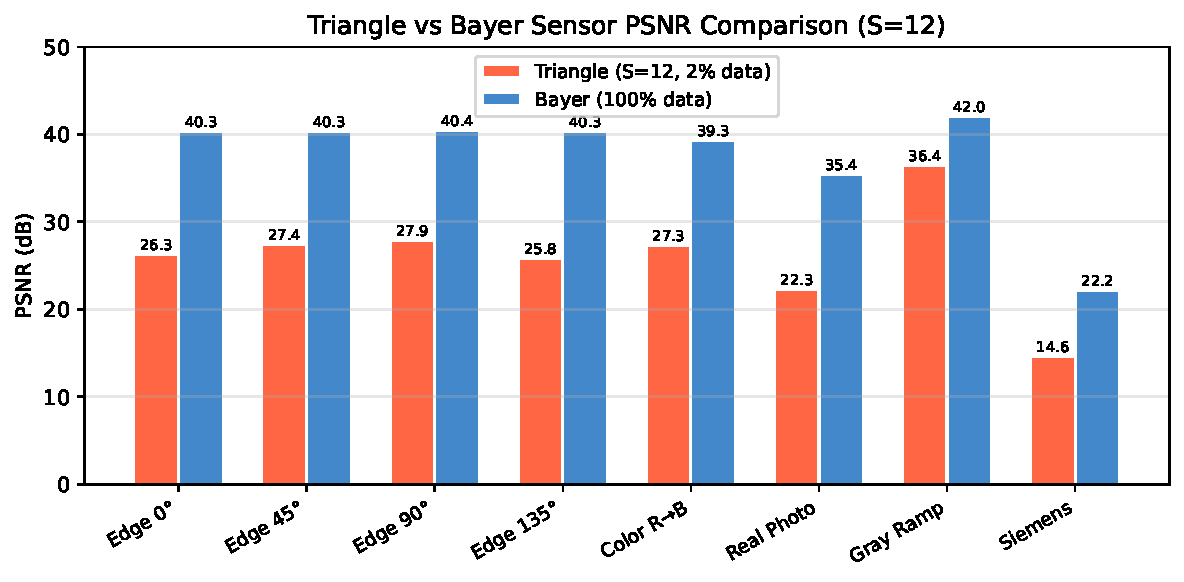
\includegraphics[width=\columnwidth]{fig3_sensor_bars.pdf}
\caption{PSNR comparison across test images. Triangle (S=12) uses 2\% of Bayer's pixel count.}
\label{fig:sensor}
\end{figure}

\textbf{Key findings:}
\begin{itemize}[nosep]
\item Directional anisotropy is only \textbf{2.1 dB} (max$-$min PSNR across orientations), demonstrating near-isotropic response despite the color pattern's 3-fold symmetry within the grid's 6-fold geometric symmetry (Fig.~\ref{fig:aniso}).
\item The 90\textdegree\ edge (aligned with the horizontal triangle axis) achieves the best PSNR (27.9 dB).
\item On smooth gradients, the triangle sensor is nearly lossless (36.4 dB, SSIM 0.999).
\item Real photograph achieves SSIM 0.905 with only 2\% data.
\end{itemize}

\begin{figure}[t]
\centering
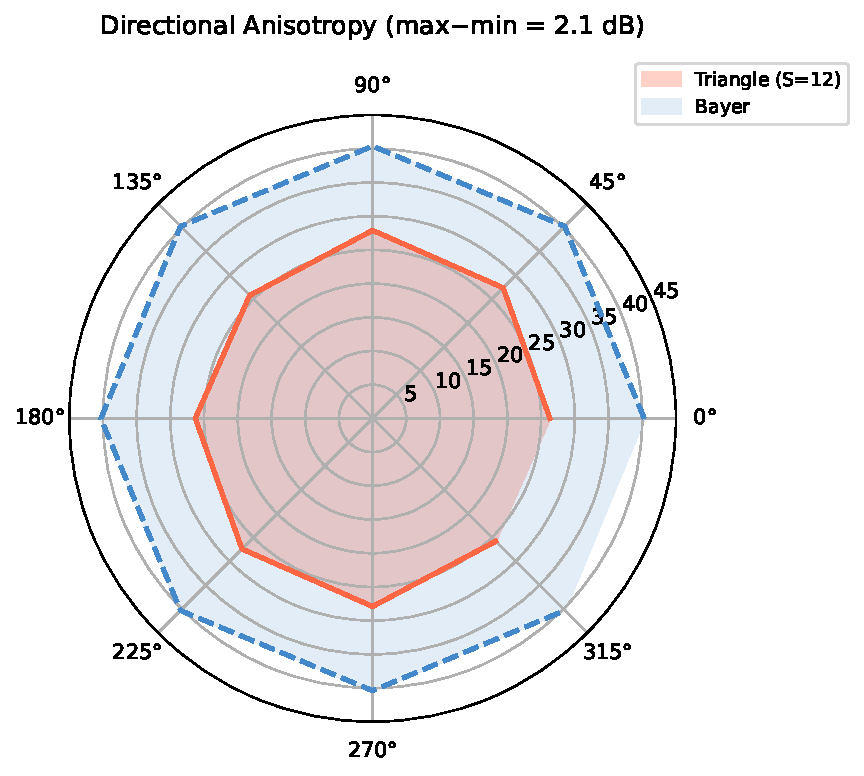
\includegraphics[width=0.85\columnwidth]{fig4_anisotropy.pdf}
\caption{Directional anisotropy radar chart. Triangle PSNR varies by only 2.1~dB across all edge orientations (Bayer: 0.1~dB).}
\label{fig:aniso}
\end{figure}

\subsection{AI vs Hand-Crafted ISP}

Figure~\ref{fig:ai} compares the 3-layer GCN ($\sim$1,300 parameters) with our hand-crafted ISP. On the edge image, the GCN achieves 24.7~dB vs.\ ISP's 25.1~dB (gap of only 0.4~dB). The GCN requires per-image training (self-supervised, 0.6--7.4~s), making it suitable for applications where per-scene optimization is acceptable.

\subsection{Processing Speed}

Table~\ref{tab:speed} shows pipeline throughput. The full pipeline (sample + borrow + ISP $\times$3 + render) achieves real-time performance at smaller triangle sizes, with 203~FPS at S=32.

\begin{table}[t]
\centering
\caption{Processing speed (numba JIT, AMD 7840)}
\label{tab:speed}
\begin{tabular}{cccc}
\toprule
Side & Triangles & Time & FPS \\
\midrule
S=16 & 1,219 & 17 ms & 59 \\
S=20 & 817 & 12 ms & 85 \\
S=24 & 576 & 8 ms & 121 \\
S=32 & 336 & 5 ms & 203 \\
\bottomrule
\end{tabular}
\end{table}

\begin{figure}[t]
\centering
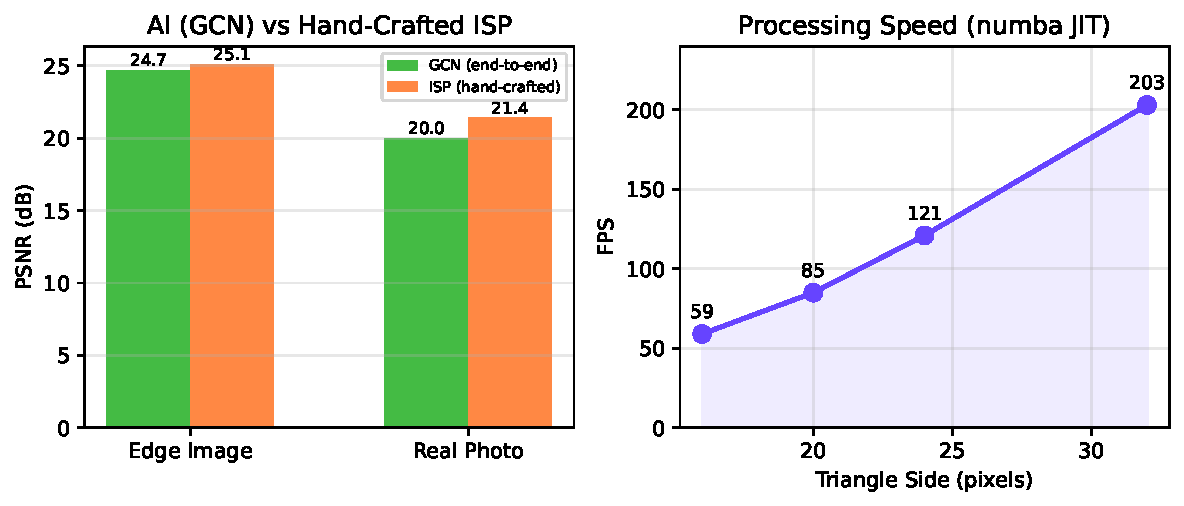
\includegraphics[width=\columnwidth]{fig5_ai_speed.pdf}
\caption{Left: GCN vs ISP PSNR comparison. Right: Pipeline throughput vs triangle size.}
\label{fig:ai}
\end{figure}

%-------------------------------------------------------------------------
\section{Discussion}
%-------------------------------------------------------------------------

\subsection{Comparison with Bayer}

At equivalent data rates (both RAW: 8 bits/pixel), the triangular sensor achieves 70\% of Bayer PSNR using 2\% of spatial samples. At S=4 (15\% data), the gap narrows to $\sim$7~dB. The advantage is data efficiency: comparable perceptual quality with fewer measurements, not raw PSNR at equal resolution.

\subsection{Limitations}

\begin{itemize}[nosep]
\item \textbf{High-frequency loss:} The Siemens star benchmark reveals detail loss at high spatial frequencies, inherent to coarser sampling.
\item \textbf{AI training:} The GCN requires per-image training; a generalizable model needs diverse data.
\item \textbf{Rendering:} PIL-based triangle rendering is the bottleneck; GPU rasterization would enable higher resolutions.
\item \textbf{Physical validation:} All results are simulation; a physical triangular CMOS sensor is needed.
\end{itemize}

\subsection{Future Work}

\begin{itemize}[nosep]
\item Physical sensor fabrication: CMOS design with triangular photodiode arrangement.
\item Video pipeline: Temporal consistency across triangular frames.
\item Learned super-resolution: Training larger GCNs on the Sierpinski pyramid.
\item Triangular SLAM: Direct 3D reconstruction from triangular keypoints.
\end{itemize}

%-------------------------------------------------------------------------
\section{Conclusion}
%-------------------------------------------------------------------------

We presented Triangle Pixel, a complete vision system replacing rectangular pixel grids with equilateral triangle meshes. The system spans sensor simulation through AI-native processing, demonstrating that triangular representations can match or exceed rectangular ones in data efficiency (70\% of Bayer PSNR at 2\% data), geometric isotropy (2.1~dB directional variation), and 3D integration, while enabling zero-computation color reconstruction and Sierpinski-based multi-scale processing at real-time speeds (59~FPS).

%-------------------------------------------------------------------------
\bibliographystyle{ieee}
\begin{thebibliography}{9}

\bibitem{bayer1976}
B.~E.~Bayer, ``Color imaging array,'' U.S. Patent 3,971,065, 1976.

\bibitem{hamilton1997}
J.~F.~Hamilton and J.~E.~Adams, ``Adaptive color plan interpolation in single sensor color electronic camera,'' U.S. Patent 5,629,734, 1997.

\bibitem{kipf2017}
T.~N.~Kipf and M.~Welling, ``Semi-supervised classification with graph convolutional networks,'' \textit{ICLR}, 2017.

\bibitem{lowe2004}
D.~G.~Lowe, ``Distinctive image features from scale-invariant keypoints,'' \textit{IJCV}, 2004.

\bibitem{harris1988}
C.~Harris and M.~Stephens, ``A combined corner and edge detector,'' \textit{Alvey Vision Conference}, 1988.

\bibitem{canny1986}
J.~Canny, ``A computational approach to edge detection,'' \textit{IEEE TPAMI}, 1986.

\bibitem{fujifilm2012}
Fujifilm, ``X-Trans CMOS sensor,'' \textit{Fujifilm Technical Review}, 2012.

\bibitem{hubel2004}
P.~M.~Hubel, J.~Liu, and R.~J.~Guttosch, ``Spatial frequency response of color image sensors: Bayer color filters and Foveon X3,'' \textit{Proc. SPIE}, 2004.

\bibitem{gharbi2016}
M.~Gharbi, G.~Chaurasia, S.~Paris, and F.~Durand, ``Deep joint demosaicking and denoising,'' \textit{ACM TOG}, 2016.

\end{thebibliography}

\end{document}
